\Variant{28.02.2026 (2-smena)}
\QQ{1}{$\underbrace{77\ldots79}_{2025\text{ ta}}+\underbrace{77\ldots78}_{2025\text{ ta}}+\underbrace{77\ldots77}_{2025\text{ ta}}+\ldots+\underbrace{77\ldots72}_{2025\text{ ta}}+\underbrace{77\ldots71}_{2025\text{ ta}}$ yiğindini $7$ ga bölgandagi qoldiqni toping.
\Opts{$1$}{$6$}{$0$}{$3$}}
\QQ{2}{Hisoblang:
\[4\frac2{2025}\cdot6\frac5{2026}-2\frac{2023}{2025}\cdot7\frac{2021}{2026}-\frac{35}{2026}\]
\Opts{$\dfrac7{1013}$}{$\dfrac7{2026}$}{$\dfrac{14}{1013}$}{$\dfrac{28}{2025}$}}
\QQ{3}{$A$ va $B$ şaharlar orasidagi masofa $24$ km. $A$ şahardan $B$ şaharga bir vaqtda ikki yölovçi yölga çiqdi. Birinçisi $1$ soatda ikkinçisidan $2$ km köp yöl bosib ötadi. Agar birinçi yölovçi ikkinçisidan $1$ soat oldin manzilga yetib kelgan bölsa, ikkinçi yölovçi neça soatda yetib kelgan?
\Opts{$4$}{$6$}{$3$}{$8$}}
\QQ{4}{Malikaning $2$ ta bir xil köylagi bor. U $1$-köylakni $5\%$ çegirma bilan va $2$-köylakni çegirmasiz sotdi. $1$-köylakdan olgan foydasi $1$-köylakning sotilgan narxining $18\%$ ga teng. $2$-köylakning foydasi sotilgan narxining neça foiziga teng?
\Opts{$23{,}1$}{$22{,}1$}{$23{,}2$}{$22$}}
\QQ{5}{Hisoblang:
\[\frac{\left(3^4\cdot2\right)^{-\frac12}}{9^{-3}\cdot2^{-2}}\]
\Opts{$162\sqrt2$}{$\dfrac{81}{2\sqrt2}$}{$\dfrac{2\sqrt2}{81}$}{$162$}}
\QQ{6}{Hisoblang:
\[\sqrt[6]{7-\sqrt{40}}\cdot\sqrt[3]{\sqrt2+\sqrt5}\cdot\sqrt[3]9\]
\Opts{$3$}{$-3$}{$6\sqrt3$}{$3\sqrt3$}}
\QQ{7}{Hisoblang:
\[\frac5{\sqrt[3]{32}+2}+\frac5{\sqrt[3]{128}-\sqrt[3]{32}+2}-\sqrt[3]2\]
\Opts{$-1$}{$1$}{$0$}{$\sqrt6$}}
\QQ{8}{Arifmetik progressiyaning umumiy hadi formulasi $a_n=3{,}8-0{,}7n$ bölsa, dastlabki ön bitta hadi yiğindisini toping.
\Opts{$-0{,}55$}{$-4{,}4$}{$-3{,}7$}{$-3{,}3$}}
\QQ{9}{Kamayuvçi geometrik progressiyada $b_1+b_2+b_3=19$ va $b_1^2+b_2^2+b_3^2=133$ bölsa, dastlabki $5$ ta hadi yiğindisini toping.
\Opts{$22\dfrac49$}{$22\dfrac59$}{$23\dfrac19$}{$23\dfrac49$}}
\QQ{10}{$a=\sqrt2$ va $b=\sqrt{18}$ bölsa, ifodaning qiymatini toping.
\[\left(\frac{\sqrt{ab}}{\sqrt a+\sqrt b}-\frac b{\sqrt b-\sqrt a}+\frac{2b\sqrt a}{a-b}\right)\cdot\left(\frac1{\sqrt a-\sqrt b}-\frac{\sqrt b}{a+\sqrt{ab}}+\frac{2\sqrt b}{b-a}\right)\]
\Opts{$9$}{$3$}{$\sqrt3$}{$\sqrt6$}}
\QQ{11}{Soddalaştiring:
\[(2x-1)^4-8x(2x-1)^3+24x^2(2x-1)^2-32x^3(2x-1)+16x^4\]
\Opts{$1$}{$(4x-1)^2$}{$\dfrac12$}{$-1$}}
\QQ{12}{Tenglamaning $\left[-\dfrac\pi2;\,\dfrac{5\pi}2\right]$ oraliqda neçta ildizi bor?
\[\cos\left(\frac{3\pi}2+2x\right)=0\]
\Opts{$3$}{$2$}{$7$}{$4$}}
\QQ{13}{Tenglama $\left[-\dfrac{3\pi}2;\,\dfrac{5\pi}2\right]$ kesmada neçta yeçimga ega?
\[\sin^4x+\cos^4x=1\]
\Opts{$8$}{$4$}{$9$}{$7$}}
\QQ{14}{Tenglamalar sistemasining yeçimi $(x;\,y)$ bölsa, $x\cdot y$ ni toping.
\[\begin{cases}x^{3y-4}=9,\\ x^{y+1}=27\end{cases}\]
\Opts{$8$}{$10$}{$9$}{$6$}}
\QQ{15}{Tenglamaning haqiqiy ildizlari neçta?
\[\frac{\sqrt{4-x}-\sqrt{5x^3-4x^2-4x}}{\sqrt{4-x}+\log_5^2\left(5x^3-4x^2+1\right)}=1\]
\Opts{Çeksiz köp yeçimga ega}{$1$}{Haqiqiy ildizga ega emas}{$2$}}
\QQ{16}{Tenglama neçta butun yeçimga ega?
\[x^4-\frac{2027!}{2026!+2025!}\,x^2+2025=0\]
\Opts{$1$ ta}{$2$ ta}{$3$ ta}{$4$ ta}}
\QQ{17}{Tenglamani yeçing:
\[x+\frac x{1+2}+\frac x{1+2+3}+\frac x{1+2+3+4}+\ldots+\frac x{1+2+3+\ldots+4041}=4041\]
\Opts{$2021$}{$2022$}{$2023$}{$2024$}}
\QQ{18}{Tengsizlikning yeçimi böladigan butun sonlar yiğindisini toping.
\[\frac{\left|x^2-8x+12\right|}{18+7x-x^2}>0\]
\Opts{$35$}{$27$}{$30$}{$24$}}
\QQ{19}{Tengsizlikni qanoatlantiruvçi butun sonlar neçta?
\[\sqrt{x^2-4x+4}<5\sqrt{2-x}+6\]
\Opts{$34$}{$36$}{$35$}{$37$}}
\QQ{20}{Funksiyaning aniqlaniş sohasiga tegişli neçta butun qiymat bor?
\[y=\log_{x+2}\frac{(x-2)\sqrt{24+2x-x^2}}{x-2}\]
\Opts{$5$ ta}{$6$ ta}{$4$ ta}{$7$ ta}}
\QQ{21}{Aniq integralni hisoblang:
\[\int_{-\frac\pi4}^{\frac\pi4}\frac{\sin^3x}{\cos^7x}\,dx\]
\Opts{$-\dfrac15$}{$0$}{$\dfrac15$}{$-\dfrac5{12}$}}
\QQ{22}{$y=\dfrac{x^4+1}{x^2+1}$ funksiyaning qiymatlar sohasini toping.
\Opts{$\left(-2\sqrt2-2;\,\infty\right)$}{$\left(-2\sqrt2-2;\,2\sqrt2-2\right)$}{$\left[2\sqrt2-2;\,\infty\right)$}{$\left(2\sqrt2;\,\infty\right)$}}
\QQ{23}{Aylananing $8$ ga teng vatari $90^\circ$ li yoyni tortib turadi. Aylana radiusini toping.
\qfig{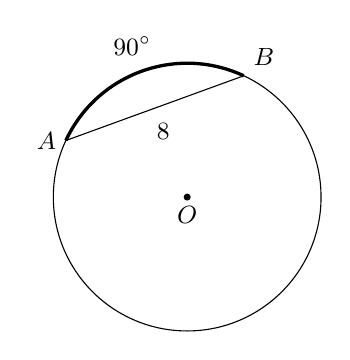
\begin{tikzpicture}[scale=0.85,font=\small]
\coordinate (O) at (0,0); \coordinate (A) at (155:2); \coordinate (B) at (65:2);
\draw (O) circle (2); \draw (A)--(B); \fill (O) circle (1.5pt);
\draw[very thick] (A) arc (155:65:2);
\node[left] at (A) {$A$}; \node[above right] at (B) {$B$}; \node[below] at (O) {$O$};
\node at (110:1.05) {$8$}; \node at (110:2.4) {$90^\circ$};
\end{tikzpicture}}
\Opts{$3\sqrt2$}{$4$}{$4\sqrt2$}{$8$}}
\QQ{24}{$f(x)=(x-8)\cdot e^{x-7}$ funksiyaning $[5;\,9]$ oraliqdagi eng kiçik qiymatini toping.
\Opts{$-1$}{$e^2$}{$-\dfrac3{e^2}$}{$0$}}
\QQ{25}{$ABC$ va $FED$ muntazam uçburçaklar berilgan. Agar $AB=18$ va $AF:FC=CD:DB=BE:EA=1:2$ bölsa, $FED$ uçburçak yuzini toping.
\qfig{\begin{tikzpicture}[scale=0.22,font=\small]
\coordinate (A) at (9,15.588); \coordinate (C) at (0,0); \coordinate (B) at (18,0);
\coordinate (F) at (6,10.392); \coordinate (D) at (6,0); \coordinate (E) at (15,5.196);
\fill[qfill] (F)--(E)--(D)--cycle; \draw (A)--(B)--(C)--cycle; \draw (F)--(E)--(D)--cycle;
\node[above] at (A) {$A$}; \node[below left] at (C) {$C$}; \node[below right] at (B) {$B$};
\node[above left] at (F) {$F$}; \node[below] at (D) {$D$}; \node[right] at (E) {$E$};
\end{tikzpicture}}
\Opts{$27\sqrt3$}{$18\sqrt3$}{$9$}{$9\sqrt3$}}
\QQ{26}{Rasmda berilganlarga asoslanib, böyalgan soha yuzini toping.
\qfig{\begin{tikzpicture}[scale=0.32,font=\small]
\coordinate (B) at (0,0); \coordinate (C) at (14,0); \coordinate (A) at (5,12); \coordinate (I) at (6,4); \coordinate (D) at (6.5,0); \coordinate (K) at (2.414,5.793);
\fill[qfill] (A)--(I)--(C)--cycle;
\draw (A)--(B)--(C)--cycle; \draw (A)--(D); \draw (C)--(K);
\draw (A)++(-112.6:1.6) arc (-112.6:-82.9:1.6); \draw (A)++(-82.9:2.0) arc (-82.9:-53.1:2.0);
\node[font=\scriptsize] at (4.6,9.6) {$\alpha$}; \node[font=\scriptsize] at (6.0,9.5) {$\alpha$};
\draw (C)++(180:2.6) arc (180:153.4:2.6); \draw (C)++(153.4:3.2) arc (153.4:126.9:3.2);
\node[font=\scriptsize] at (10.8,0.75) {$\beta$}; \node[font=\scriptsize] at (11.1,2.45) {$\beta$};
\node[above right] at (9.5,6) {$15$}; \node[below] at (3.25,0) {$6{,}5$}; \node[below] at (10.25,0) {$7{,}5$};
\end{tikzpicture}}
\Opts{$15\sqrt3$}{$14\sqrt3$}{$28$}{$30$}}
\QQ{27}{Asoslari $3$ va $9$ bölgan töğri burçakli trapetsiyaning kiçik yon tomoni $6$ ga teng. Trapetsiyaning diagonallari kesişiş nuqtasidan katta asosgaça bölgan masofani toping.
\qfig{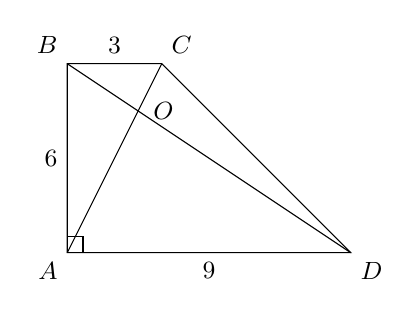
\begin{tikzpicture}[scale=0.4,font=\small]
\coordinate (A) at (0,0); \coordinate (D) at (9,0); \coordinate (B) at (0,6); \coordinate (C) at (3,6); \coordinate (O) at (2.25,4.5);
\draw (A)--(B)--(C)--(D)--cycle; \draw (A)--(C); \draw (B)--(D); \draw (0,0.5)--(0.5,0.5)--(0.5,0);
\node[below left] at (A) {$A$}; \node[above left] at (B) {$B$}; \node[above right] at (C) {$C$}; \node[below right] at (D) {$D$}; \node[right=2pt] at (O) {$O$};
\node[above] at (1.5,6) {$3$}; \node[below] at (4.5,0) {$9$}; \node[left] at (0,3) {$6$};
\end{tikzpicture}}
\Opts{$4{,}5$}{$3$}{$3{,}5$}{$1$}}
\QQ{28}{Muntazam köpburçakning diagonallari soni $35$ ta bölsa, uning bir uçidan çiqqan eng katta va eng kiçik diagonallari orasidagi burçakni toping.
\Opts{$54^\circ$}{$72^\circ$}{$45^\circ$}{$60^\circ$}}
\QQ{29}{$A(3;\,1;\,2)$, $B(-1;\,1;\,4)$ va $C(0;\,2;\,2)$ — uçburçakning uçlari. $C$ uçidan $AB$ tomonga tuşirilgan mediana uzunligini toping.
\Opts{$\sqrt{10}$}{$\sqrt{20}$}{$\sqrt6$}{$\sqrt3$}}
\QQ{30}{Muntazam oltiburçakli piramidaning yon qirrasi asos tekisligi bilan $60^\circ$ li burçak hosil qiladi. Agar yon qirrasining uzunligi $\sqrt{39}$ bölsa, piramidaning hajmini toping.
\Opts{$13$}{$\dfrac{117\sqrt{39}}{32}$}{$\dfrac{39\sqrt{39}}{32}$}{$\dfrac{117\sqrt{39}}{16}$}}
\QQ{31}{Rasmdagi sonlar töplamlarning elementlari. $(A\cup C)\cap(B\cup D)$ töplamning elementlari sonini toping.
\qfig{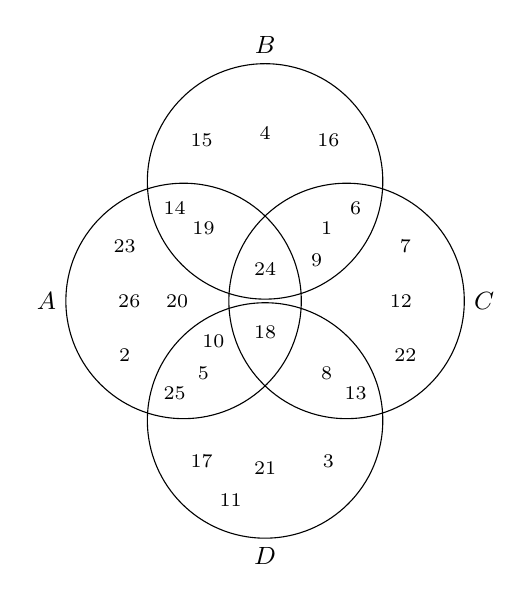
\begin{tikzpicture}[scale=1.15,font=\scriptsize]
\draw (-0.9,0) circle (1.3); \draw (0,1.32) circle (1.3); \draw (0.9,0) circle (1.3); \draw (0,-1.32) circle (1.3);
\node[left,font=\small] at (-2.2,0) {$A$}; \node[above,font=\small] at (0,2.62) {$B$}; \node[right,font=\small] at (2.2,0) {$C$}; \node[below,font=\small] at (0,-2.62) {$D$};
\node at (0.00,1.85) {4}; \node at (-0.70,1.77) {15}; \node at (0.70,1.77) {16}; \node at (0.68,0.80) {1}; \node at (1.00,1.02) {6}; \node at (0.57,0.45) {9}; \node at (-0.68,0.80) {19}; \node at (-1.00,1.02) {14}; \node at (0.00,0.35) {24}; \node at (-1.50,0.00) {26}; \node at (-1.55,-0.60) {2}; \node at (-1.55,0.60) {23}; \node at (-0.97,0.00) {20}; \node at (1.50,0.00) {12}; \node at (1.55,-0.60) {22}; \node at (1.55,0.60) {7}; \node at (-0.68,-0.80) {5}; \node at (-1.00,-1.02) {25}; \node at (-0.57,-0.45) {10}; \node at (0.00,-0.35) {18}; \node at (0.68,-0.80) {8}; \node at (1.00,-1.02) {13}; \node at (0.00,-1.85) {21}; \node at (-0.70,-1.77) {17}; \node at (0.70,-1.77) {3}; \node at (-0.38,-2.20) {11};
\end{tikzpicture}}
\Opts{$12$}{$11$}{$13$}{$16$}}
\QQ{32}{«MATEMATIKA» sözidagi har bir harf bittadan qoğozga yozib çiqildi. Bitta qoğoz olinganda M harfi çiqiş ehtimolini toping.
\Opts{$\dfrac1{10}$}{$\dfrac3{10}$}{$\dfrac15$}{$\dfrac25$}}
\QQ{33}{\Moslash{Muntazam uçburçakli piramidaga konus içki çizilgan, konus asosining radiusi $4$ ga teng. Piramidaning yon yoqlari asos tekisligi bilan $60^\circ$ li burçak hosil qiladi ($\pi\approx3$ deb olinsin).}{A) $48$\par B) $96$\par C) $192$\par D) $64\sqrt3$\par E) $96\sqrt3$\par F) $100$}{Konus yon sirti yuzini toping.}{Piramidaning yon sirti yuzini toping.}{Piramidaning hajmini toping.}}
\QQ{36}{Tenglamalar sistemasini yeçing:
\[\begin{cases}x-\frac14xy-y=0,\\[2pt] x^2-\frac52xy+y^2=0\end{cases}\]
\AB{Agar tenglamalar sistemasi yeçimlari $(x_1;y_1)$, $(x_2;y_2)$, \dots, $(x_n;y_n)$ bölsa, $x_n\cdot y_n$ ning eng katta qiymatini toping.}{Tenglamalar sistemasi neçta yeçimga ega?}}
\QQ{37}{Tenglamani yeçing:
\[\sin^2x+\sin2x=3\cos^2x\]
\AB{Tenglamaning eng katta manfiy yeçimini toping.}{Tenglamaning $[-\pi;\,\pi]$ oraliqdagi yeçimlari sonini toping.}}
\QQ{38}{$f(x)$ va $g(x)$ funksiyalar uçun $f(3x-2)+7\cdot g(x-5)=x+1$ va $f(x+1)-g\left(\dfrac x3-4\right)=3x$ bölsa,
\AB{$\bigl(f(1)\bigr)^{-1}$ ni toping.}{$f(x)+g(x)=\dfrac12$ tenglamaning ildizlari sonini toping.}}
\QQ{39}{Quyidagi rasmda $f(x)$ funksiyaning grafigi tasvirlangan.
\qfig{\begin{tikzpicture}[xscale=0.62,yscale=0.62,font=\scriptsize]
\draw[-{Stealth[length=4pt]}] (-10,0)--(6,0) node[right] {$x$}; \draw[-{Stealth[length=4pt]}] (0,-2.4)--(0,3.8) node[left] {$y$};
\draw[thick] plot[smooth,tension=0.6] coordinates {(-9,2.6) (-8.6,0.0) (-8,-1.6) (-7.5,-1.15) (-7,-1.0) (-6.5,-1.4) (-6,-2.0) (-5.55,1.0) (-5,3.1) (-4.5,1.6) (-4,0) (-3.5,-1.15) (-3,-1.45) (-2.5,-1.05) (-2,-0.2) (-1,1.9) (0,2.8) (1,1.6) (2,0.4) (3,1.7) (4,2.8) (4.5,1.3) (5,-1.3)};
\foreach \a/\b in {-9/2.6,-8/-1.6,-7/-1.0,-6/-2.0,-5/3.1,2/0.4,4/2.8,5/-1.3} \draw[dashed] (\a,0)--(\a,\b);
\foreach \a in {-9,-7,-5,2,4} \node[below] at (\a,0) {$\a$};
\foreach \a in {-8,-6,5} \node[above] at (\a,0) {$\a$};
\node[above right] at (-4,0) {$-4$}; \node[above left] at (-2,0) {$-2$}; \node[below left] at (0,0) {$O$};
\end{tikzpicture}}
\AB{$[-9;\,5]$ kesmada $f(x)$ funksiyaning ekstremum nuqtalari neçta?}{$[-9;\,5]$ kesmada $f'(x)<0$ tengsizlikni qanoatlantiradigan butun qiymatlar neçta?}}
\QQ{40}{$f(x)=px^2+qx$ va $g(x)=ax^3+bx^2+cx$ funksiyalar berilgan. Bu funksiyalar $(-2;\,-8)$ va $(2;\,0)$ nuqtalarda kesişadi, bunda $g(x)$ funksiya grafigi $\left(-1\frac23;\,0\right)$ nuqtadan ötadi.
\qfig{\begin{tikzpicture}[xscale=1.25,yscale=0.24,font=\scriptsize]
\fill[qfill] plot[domain=-2:2,samples=80] (\x,{3*\x*\x*\x-\x*\x-10*\x}) -- plot[domain=2:-2,samples=60] (\x,{-\x*\x+2*\x}) -- cycle;
\draw[-{Stealth[length=4pt]}] (-2.8,0)--(3.2,0) node[right] {$x$}; \draw[-{Stealth[length=4pt]}] (0,-11)--(0,10) node[left] {$y$};
\draw[thick] plot[domain=-2.08:2.27,samples=100] (\x,{3*\x*\x*\x-\x*\x-10*\x}) node[right] {$y=g(x)$};
\draw[thick] plot[domain=-2.2:2.9,samples=60] (\x,{-\x*\x+2*\x}) node[below right] {$y=f(x)$};
\fill (-2,-8) circle (1.5pt); \fill (2,0) circle (1.5pt); \fill (-1.667,0) circle (1.5pt);
\node[left=3pt] at (-2,-8) {$(-2;\,-8)$}; \node[above right] at (2,0) {$2$}; \node[above left] at (-1.667,0) {$-\frac53$}; \node[below left] at (0,0) {$O$};
\end{tikzpicture}}
\AB{$\dfrac{a+b+c}{p+q}$ ni toping.}{Böyalgan soha yuzini toping.}}
\QQ{41}{$ABC$ töğri burçakli uçburçakka $O$ markazli aylana içki çizilgan. $CO$ töğri çiziq $AB$ gipotenuzani $D$ nuqtada kesib ötadi. Agar içki çizilgan aylana radiusi $\sqrt3$ ga va $CO:OD=\sqrt3:\sqrt2$ bölsa,
\qfig{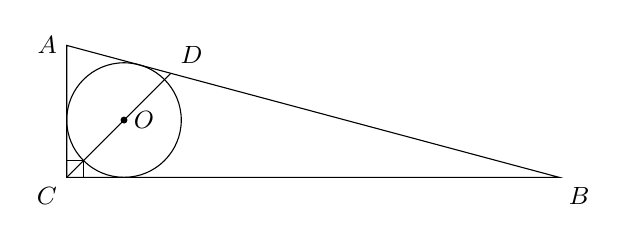
\begin{tikzpicture}[scale=0.42,font=\small]
\coordinate (C) at (0,0); \coordinate (B) at (14.888,0); \coordinate (A) at (0,3.989); \coordinate (O) at (1.732,1.732); \coordinate (D) at (3.146,3.146);
\draw (A)--(B)--(C)--cycle; \draw (O) circle (1.732); \draw (C)--(D); \fill (O) circle (3pt);
\draw (0,0.5)--(0.5,0.5)--(0.5,0);
\node[left] at (A) {$A$}; \node[below left] at (C) {$C$}; \node[below right] at (B) {$B$}; \node[above right] at (D) {$D$}; \node[right] at (O) {$O$};
\end{tikzpicture}}
\AB{$OD$ kesma uzunligini toping.}{Töğri burçakli uçburçakning kiçik burçagini toping.}}
\QQ{42}{Ikkita kvadrat rasmdagi körinişda çizildi. Agar $S_1=9$ va $S_2=27$ bölsa,
\qfig{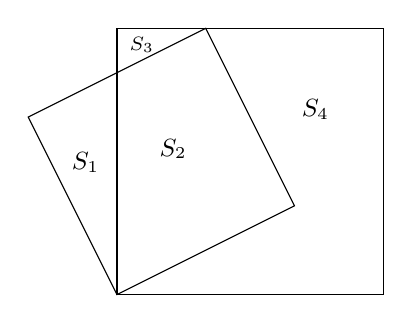
\begin{tikzpicture}[scale=0.42,font=\small]
\coordinate (P) at (0,0); \coordinate (R) at (5.367,2.683); \coordinate (T) at (-2.683,5.367); \coordinate (Q) at (2.683,8.050);
\draw (0,0) rectangle (8.05,8.05); \draw (P)--(R)--(Q)--(T)--cycle;
\node at (-0.95,4.0) {$S_1$}; \node at (1.7,4.4) {$S_2$}; \node[font=\scriptsize] at (0.75,7.55) {$S_3$}; \node at (6,5.6) {$S_4$};
\end{tikzpicture}}
\AB{$S_3$ ni toping.}{$S_4$ ni toping.}}
\QQ{43}{Tomonining uzunligi $9$ ga teng bölgan $ABCDEF$ muntazam oltiburçakning $BC$ tomonidan $G$ nuqta, $AF$ tomonidan $H$ nuqta olindi. Agar $BG=1$ va $HF=2$ bölsa, rasmdagi maʼlumotlar asosida
\qfig{\begin{tikzpicture}[scale=0.3,font=\small]
\coordinate (A) at (0,0); \coordinate (F) at (9,0); \coordinate (E) at (13.5,7.794); \coordinate (D) at (9,15.588); \coordinate (C) at (0,15.588); \coordinate (B) at (-4.5,7.794);
\coordinate (G) at (-4,8.66); \coordinate (H) at (7,0);
\draw (A)--(B)--(C)--(D)--(E)--(F)--cycle; \draw (G)--(H);
\node[below left] at (A) {$A$}; \node[left] at (B) {$B$}; \node[above left] at (C) {$C$}; \node[above right] at (D) {$D$}; \node[right] at (E) {$E$}; \node[below right] at (F) {$F$};
\node[above left] at (G) {$G$}; \node[below] at (H) {$H$}; \node[left,font=\scriptsize] at (-4.25,8.3) {$1$}; \node[below,font=\scriptsize] at (8,0) {$2$};
\node at (-0.6,4.0) {$S_1$}; \node at (6,9.5) {$S_2$};
\end{tikzpicture}}
\AB{$GH$ kesma uzunligini toping.}{$\dfrac{S_1}{S_2}$ ni toping.}}
\QQ{44}{$ABCD$ piramidada $D$ — piramidaning uçi, $DC$ qirrasi $3$ ga teng. Radiusi $\dfrac23$ ga teng bölgan sfera piramidaning $ABD$ yon yoğiga, $DC$ qirrasiga va $ABC$ uçburçakka uning medianalari kesişgan nuqtasida urinadi. Agar $AD$ qirrasi $ABC$ yoğiga perpendikulyar va $AC=BC$ bölsa,
\AB{$ABC$ uçburçakning $AB$ tomoniga tuşirilgan medianasi uzunligini toping.}{Piramida hajmini toping.}}
\QQ{45}{Korxona rahbari korxonaga ketadigan xarajatlarni hisoblab çiqdi. Bunda korxonaning daromad funksiyasi $A(x)=\dfrac{2x}3$, xarajat funksiyasi esa $B(x)=2\sqrt x$, bu yerda $x$ — işçilar soni.
\AB{Korxona zarar körmasligi uçun kamida neçta işçi olişi kerak?}{Korxona foyda körişi uçun eng kamida neçta işçi olişi kerak?}}
\Javoblar{D D A B A A B B D C A C C D B D A B B A B C C A A D A A D D A C B E C}{\OK{36}{$8$}{$3$}\OK{37}{$-\arctg3$}{$4$}\OK{38}{$4$}{$1$}\OK{39}{$8$}{$4$}\OK{40}{$-8$}{$24$}\OK{41}{$2$}{$15^\circ$}\OK{42}{$\dfrac95$}{$36$}\OK{43}{$14$}{$\dfrac{79}{407}$}\OK{44}{$2$}{$\dfrac43$}\OK{45}{$9$}{$10$}}
